
%%%%%%%%%%%%%%%%%%%%%%%%%%%%%%%%%%%%%%%%%%%%%%%%%%%%%%%%%%%%%%%%%%%%%%%%%%%



\documentclass[a4,compress,handout]{beamer}
\usepackage{beamerthemesplit}
\usepackage{ae}
\usepackage{graphicx}
\graphicspath{ {poze/} }
\usepackage{mathtools}
\usepackage{float}
\usepackage{amssymb}
\usepackage{braket}
\usepackage{subcaption}
\usepackage{cite}
\usepackage{rotating}
\usepackage{url}

\usepackage[utf8x]{inputenc}


\usepackage{color}
\definecolor{darkblue}{rgb}{0.2,0.2,0.6}
\definecolor{darkdarkblue}{rgb}{0.12,.03,0.51}
\definecolor{pale}{rgb}{1,0.99,0.85}
\definecolor{lightblue}{rgb}{0.75,0.82,0.9}


\mode<presentation>
{
  \usetheme{Warsaw}%{Singapore}%{Warsaw}%{Malmoe}%{Copenhagen}%{Boadilla}
  %\usefonttheme[onlylarge]{structuresmallcapsserif}
  %\setbeamercovered{transparent}  \setbeamercovered{white}
  %\setbeamercolor{frametitle}{fg=black,bg=white}
}

\newcommand{\brosu}{\item[\color{red}$\bullet$]} 

\useinnertheme{rounded}


\newcommand{\ab}{\u{a}} 
\newcommand{\ac}{\^{a}} 
\newcommand{\ib}{\^{\i}} 
\newcommand{\tb}{\c{t}} 
\newcommand{\st}{\c{s}}
\newcommand{\Ab}{\u{A}} 
\newcommand{\Ai}{\^{A}} 
\newcommand{\Ib}{\^{I}} 
\newcommand{\Tb}{\c{T}}
\newcommand{\St}{\c{S}}

\newcommand{\dob}{,,\textit{doubling}''}
\newcommand{\fol}{,,\textit{folding}''}
\newcommand{\str}{,,\textit{stretching}''}
\newcommand{\pit}{,,\textit{pitchfork}''}
\newcommand{\nn}{$N_-/N_+$}
\newcommand{\ly}{Lyapunov}
\newcommand{\dinf}{$d_\infty$}
\newcommand{\del}{$\delta$}
\newcommand{\alf}{$\alpha$}
\newcommand{\lam}{$\lambda$}
\newcommand{\ro}{$\rho$}
\newcommand{\npmd}{$N^-_\delta/N^+_\delta$}

\setlength{\leftmargini}{0pt}

%\numberwithin{equation}{section}
%\numberwithin{figure}{section}

\renewcommand*{\thefootnote}{[\arabic{footnote}]}



\addtobeamertemplate{title page}{
\includegraphics[width=1.3cm]{siglaUB} \hfill 
\includegraphics[width=1.6cm]{siglaFFB}}{}
\title[Titlul scurt]{Titlul complet al lucrarii}
\subtitle{Lucrare de licență}
       
       
\author{Prenume NUME \\
\hspace{6cm} {\small	Conduc\u{a}tor \c{s}tiin\c{t}ific:} \\
\hspace{6.35cm} {\small Lect.\ dr.\ Roxana ZUS} \\
\hspace{6.35cm} {\small Prof.\ dr.\ Virgil B\Ab RAN}}

\institute{Universitatea din Bucure\c{s}ti \\
	Facultatea de Fizic\u{a} }
\date{\small  Bucure\c{s}ti, 30 iunie 2017}


\begin{document}


%%%%%%%%%%%%%%%%%%%% slide 1  %%%%%%%%%%%%%%%%%%%%%%%%%%%%%%%%%%%%%%


\begin{frame}
\frametitle{}
 \setbeamercolor{title}{fg=darkdarkblue,bg=lightblue}
\setbeamercolor{date}{fg=darkdarkblue,bg=lightblue}
 \titlepage
\end{frame}


%%%%%%%%%%%%%%%%%%%% slide 2  %%%%%%%%%%%%%%%%%%%%%%%%%%%%%%%%%%%%%%


\begin{frame}%[plain]
  \frametitle{Cuprins}
  \small
  \tableofcontents[hideallsubsections,pausesections]
\end{frame}





%% De aici incepi construirea prezentarilor

%%%%%%%%%%%%%%%%%%%%%%%%%%%%%%%%%%%%%%%%%%%%%%%%%%%%%%%%%%%%%%%%%%%%%%%%%%%
%                                                                         %
%                       section:  Introduction                          %
%                                                                         %
%%%%%%%%%%%%%%%%%%%%%%%%%%%%%%%%%%%%%%%%%%%%%%%%%%%%%%%%%%%%%%%%%%%%%%%%%%%


\section[Intro]{Introducere \st i motiva\tb ie}
%\tableofcontents[currentsection]
%\subsection{Motivation}

%%%%%%%%%%%%%%%%%%%% slide  3 %%%%%%%%%%%%%%%%%%%%%%%%%%%%%%%%%%%%

\begin{frame}
	\frametitle{Istoric}
	
	
	\begin{columns}[c]
		\begin{column}{0.7\textwidth}
			% \begin{block}<1->
			\centering{\color{blue}Repere } 			
			\begin{itemize}
				\item { \small sec.\ XVII:  I.\ Newton, J.\ Kepler}
				\item  { \small sec.\ XIX: P.S.\ Laplace, {\color{blue}H.\ Poincar\'{e}:} }{\it \color{darkblue} haos}
				\item anii '50-'60: 
				\begin{itemize}
					\item  	teorema Kolmogorov-Arnold-Moser
					\item E.N.\ Lorenz: {\it \color{darkblue} atractor haotic}
				\end{itemize}
				\item anii '70: 
				\begin{itemize}
					\item  	D.\ Ruelle, F.\ Takens: {\it \color{darkblue} atractor straniu}
					\item R.\ May: 
					{\it \color{darkblue} aplica\tb ia logistic\ab\ }
					\item M.J.\ Feigenbaum:
					{\it \color{darkblue} universalitatea aplica\tb iilor}
					\item B.\ Mandelbrot:
					{\it \color{darkblue} fractali}
				\end{itemize}	 
			\end{itemize}
			
		\end{column}
		%\pause
		\begin{column}{0.3\textwidth}
			
			\centering{\tiny \bf \color{darkblue} Atractorul straniu Lorenz }
			
			\hfill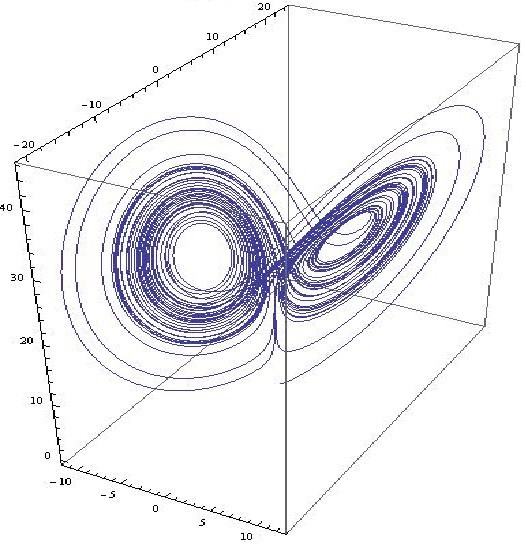
\includegraphics[width=0.8\textwidth]{lorenzstrangeatractor}\hspace*{\fill}
			
			\centering{\tiny \bf \color{darkblue} Mandelbrot set }
			
			\hfill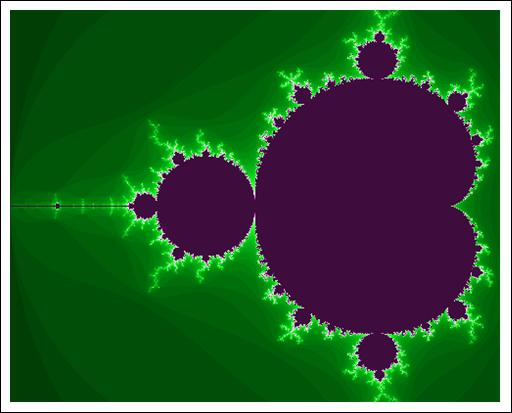
\includegraphics[width=0.6\textwidth]{mandelbrot}\hspace*{\fill}
		
		\end{column}
	\end{columns}
	\vspace{0.2cm}
	%\pause
	
	\begin{itemize}
		\item {\small J.\ Gleick: {\color{darkblue},,\textit{unde \ib ncepe haosul, \st tiin\tb a clasic\ab\ se opre\st te}"}, rezum\ab\ descoperirea lui M.J.\ Feigenbaum (1975) prin afirma\tb ia  {\color{darkblue},,o descoperire \st ocant\ab\ a faptului, c\ab , exist\ab\ structuri \ib n sistemele neliniare care sunt \ib ntotdeauna acelea\st i, dac\ab\ sunt privite din direc\tb ia potrivit\ab"}}\footnote{James Gleick, {\it Chaos: Making a new Science}, Penguin Books,  2008}.
	\end{itemize}
	
\end{frame}



%%%%%%%%%%%%%%%%%%%%% slide 4 %%%%%%%%%%%%%%%%%%%%%%%%%%%%%%%%%%%%%%

\begin{frame}
	\frametitle{Motiva\tb ie}
	\begin{itemize}
			
			\item \small \Ib n ultima jum\ab tate de secol s-au f\ab cut eforturi pentru a stabili care sunt condi\tb iile necesare ca un sistem neliniar s\ab\ prezinte comportament haotic \st i care sunt m\ab rimile potrivite pentru caracterizarea mi\st c\ab rii haotice.\end{itemize}
		%\pause
			
			Scopul tezei:
			
		\begin{itemize}
		
			\item noi {\color{darkblue} metode de caracterizare a} mecanismelor  care stau la baza {\color{darkblue} mi\st c\ab rii haotice} (aplica\tb iilor unidimensionale);
			
			%\pause 
			
			\item utilizarea {\color{red} statisticii inverse} \ib n studiul dinamicii:
			\begin{itemize}
				\brosu haotice (aplica\tb iilor unidimensionale);
				\brosu sistemului complex reprezentat de zona seismic\ab\  Vrancea (Rom\ac nia).
			\end{itemize}
		\end{itemize}
	
	
\end{frame}



%%%%%%%%%%%%%%%%%%%%%%%%%%%%%%%%%%%%%%%%%%%%%%%%%%%%%%%%%%%%%%%%%%%%%%%%%%%
%                                                                         %
%                       capitolul 2:  Caracterizarea dinamicii haotice pentru sisteme descrise de aplica\tb ii unidimensionale                          %
%                                                                         %
%%%%%%%%%%%%%%%%%%%%%%%%%%%%%%%%%%%%%%%%%%%%%%%%%%%%%%%%%%%%%%%%%%%%%%%%%%%

\section[No\tb iuni]{Caracterizarea dinamicii haotice pentru sisteme descrise de aplica\tb ii unidimensionale}
\tableofcontents[currentsection,hideallsubsections]

\subsection[No\tb iuni]{Scurt\ab\ introducere a no\tb iunilor fundamentale}

%%%%%%%%%%%%%%%%%%%%% slide 5 %%%%%%%%%%%%%%%%%%%%%%%%%%%%%%%%%%%%%%
\begin{frame}
	\frametitle{Scurt\ab\ introducere a no\tb iunilor fundamentale}
	
	
	\begin{columns}[c]
		\begin{column}{0.6\textwidth}
			
			
			\begin{itemize}
				\item { \small sec.\ XIX: T.R.\ Malthus, P.-F.\ Verhulst: primele modele de cre\st tere demografic\ab;}
				\item modelul de cre\st tere logistic:
				{\footnotesize
				\begin{equation*}
				\frac{\text{d}x}{\text{d}t}=rx\left(1-\frac{x}{k}\right),
				\end{equation*}
				}
				{\footnotesize
				\begin{equation*}
				x(t)=\frac{k}{1+C e^{-Rt}}, \text{ cu }C=\frac{k-x(0)}{x(0)};
				\end{equation*}
				}
				\item form\ab\ discret\ab\ a ecua\tb iei logistice diferen\tb iale R. May:
				\begin{equation*}
				X_{t+1}=aX_{t}\left( 1-X_{t}\right) . 
				\end{equation*}		 
			\end{itemize}
			
		\end{column}
	
		\begin{column}{0.4\textwidth}
			
			\hfill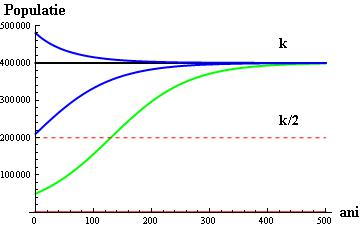
\includegraphics[width=0.99\textwidth]{20x1logcontex.jpg}\hspace*{\fill}
			
			\centering{\small \color{darkblue} Cre\st tere demografic\ab\ exponen\tb ial\ab\ \\ \tiny
				pentru rata de cre\st tere $r=0.15$, maximul demografic $k=400000$ \st i popula\tb ia ini\tb ial\ab\ $x_0=0,\ 50000,\ 210000,\ 400000,\ 480000$.}	
			
			
		\end{column}
	\end{columns}
	
\end{frame}

%%%%%%%%%%%%%%%%%%%%% slide 6 %%%%%%%%%%%%%%%%%%%%%%%%%%%%%%%%%%%%%%


\subsection[Evolu\tb ie]{Scenariul general privind evolu\tb ia dinamicii  aplica\tb iei logistice \ib n func\tb ie de parametrul de control}
\begin{frame}
	\frametitle{Scenariul general privind evolu\tb ia dinamicii  aplicatiei logistice \ib n func\tb ie de parametrul de control}
	\begin{itemize}
		\item \small Pornind de la $
		\dot{x}=rx\left(1-x \right)$,
		\item \small ob\tb inem aplica\tb ia  unidimensional\ab\ p\ab tratic\ab:
		\begin{equation*}
		x_{n+1}=r x_n  \left(1 - x_n \right)= f(x_n),
		\end{equation*}
		\ib n care $r$ este un parametru extern, de control, iar  evolu\tb ia lui $x_n$ este redus\ab\ pe intervalul $[0,1]$.
		\pause
		\item \small Rescriem  $x_{n+1}=r x_n  - r x_n^2$ \st i observ\ab m c\ab\ termenul {\color{red} $r x_n$} ac\tb ioneaz\ab\ ca {\color{red}motorul de cre\st tere} al popula\tb iei, pe c\ac nd {\color{blue}$-r x_n^2$} ca un {\color{blue}factor de diminuare} a acesteia. 
		\item \small Studiul se face pe intervalul $0 \le x_n \le 1$ deoarece o popula\tb ie negativ\ab\ nu ar avea sens.	
	\end{itemize}
	
\end{frame}


%%%%%%%%%%%%%%%%%%%%% slide 7 %%%%%%%%%%%%%%%%%%%%%%%%%%%%%%%%%%%%%%


\begin{frame}
	\frametitle{Studiul stabilit\ab\tb ii}
	\begin{itemize}
		\item Apari\tb ia, stabilitatea \st i dispari\tb ia ciclului 2: 
		{\footnotesize
			\begin{equation*}
			x_{n+1}=r x_n  \left(1 - x_n \right)= f(x_n),
			\end{equation*}}
		{\footnotesize
		\begin{equation*}
		\label{228}
		f'(x^*)= r (1- 2 x^*).
		\end{equation*}}
	\end{itemize}
	\begin{columns}[c]
		\begin{column}{0.3\textwidth}
			% \begin{block}<1->
			\hfill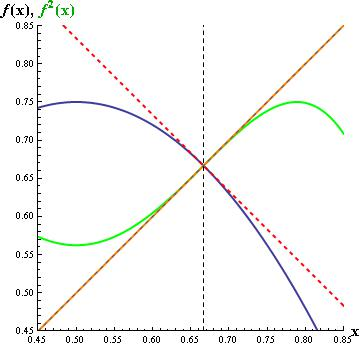
\includegraphics[width=0.9\textwidth]{229a.jpg}\hspace*{\fill}
			
			\centering{\tiny \bf \color{darkblue} Apari\tb ia ciclului 2 la $r=3$.}
			
		\end{column}
		%\pause
		\begin{column}{0.3\textwidth}
			% \begin{block}<1->
			\hfill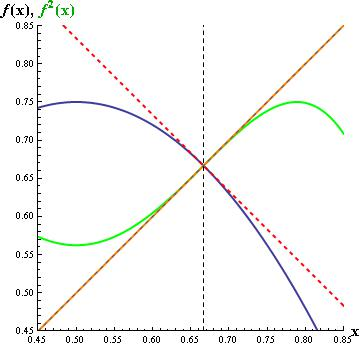
\includegraphics[width=0.9\textwidth]{229a.jpg}\hspace*{\fill}
			
			\centering{\tiny \bf \color{darkblue} Ciclul 2 superstabil la $r=1+\sqrt{5}$.}
			
		\end{column}
		%\pause
		\begin{column}{0.4\textwidth}
			% \begin{block}<1->
			\hfill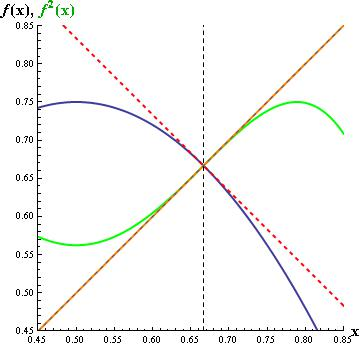
\includegraphics[width=0.9\textwidth]{229a.jpg}\hspace*{\fill}
			
			\centering{\tiny \bf \color{darkblue} Dispari\tb ia  ciclului 2 la $r=1+\sqrt{6}$.}
			
		\end{column}		
	\end{columns}	
	{\footnotesize
	\begin{equation*}
	\label{227}
	\left\{
	\begin{aligned}
	x^* & = 0, \ \text{ independent de } r; \\
	x^* & = 1 - \frac{1}{r}, \ 
	\begin{split}
	&\text{ solu\tb ie care nu are sens pentru domeniul de defini\tb ie al lui} \ x \\
	& \text{ dec\ac t dac\ab\ } 1\le r \le 4.  
	\end{split}
	\end{aligned}
	\right.
	\end{equation*}  
	}
	
\end{frame}

%%%%%%%%%%%%%%%%%%%%% slide 8 %%%%%%%%%%%%%%%%%%%%%%%%%%%%%%%%%%%%%%





\subsection[Aplica\tb ia]{Aplica\tb ia logistic\ab\ \ib n regim haotic}
\begin{frame}
	\frametitle{Aplica\tb ia logistic\ab\ \ib n regim haotic}
		\begin{columns}[c]
			\begin{column}{0.5\textwidth}
				% \begin{block}<1->
				\hfill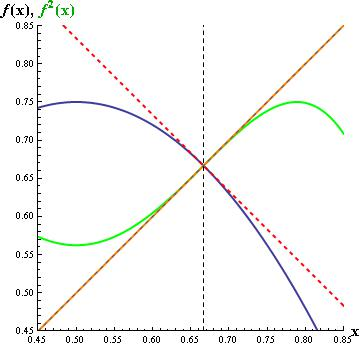
\includegraphics[width=0.7\textwidth]{229a.jpg}\hspace*{\fill}
				
				\centering{\tiny \bf \color{darkblue} Diagrama orbitelor $r \in [3.4,4]$.}
				
			\end{column}
			%\pause
			\begin{column}{0.5\textwidth}
				% \begin{block}<1->
				\hfill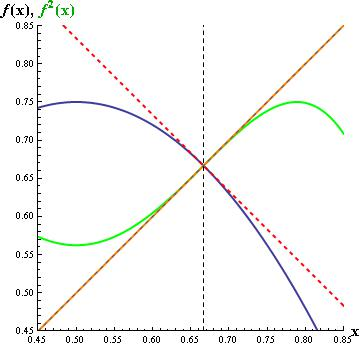
\includegraphics[width=0.7\textwidth]{229a.jpg}\hspace*{\fill}
				
				\centering{\tiny \bf \color{darkblue} Detaliu pentru $r \in [3.846, 3.858]$ \st i $x_n \in [0.13,0.18]$.}
				
			\end{column}		
		\end{columns}
		
		\begin{columns}[c]
			\begin{column}{0.33\textwidth}
				% \begin{block}<1->
				\hfill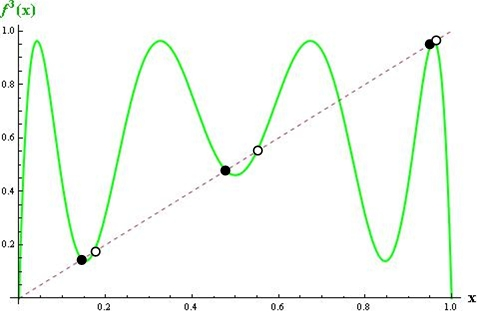
\includegraphics[width=0.9\textwidth]{232perioada3.jpg}\hspace*{\fill}
				
				\centering{\tiny \bf \color{darkblue} Perioad\ab 3 $r\gtrapprox 1+\sqrt{8}$.}
				
			\end{column}
			%\pause
			\begin{column}{0.33\textwidth}
				% \begin{block}<1->
				\hfill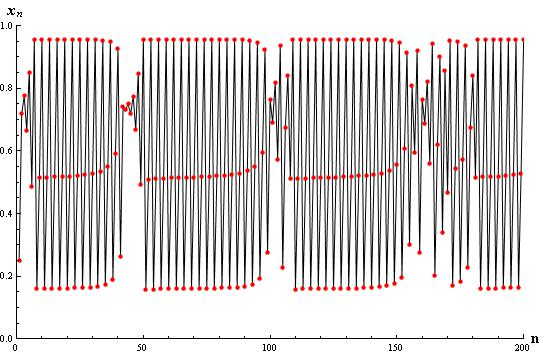
\includegraphics[width=0.9\textwidth]{234Intermitenta.jpg}\hspace*{\fill}
				
				\centering{\tiny \bf \color{darkblue} Comportamentul aplica\tb iei logistice pentru $r \lessapprox 1+\sqrt{8}$.}
				
			\end{column}
			%\pause
			\begin{column}{0.33\textwidth}
				% \begin{block}<1->
				\hfill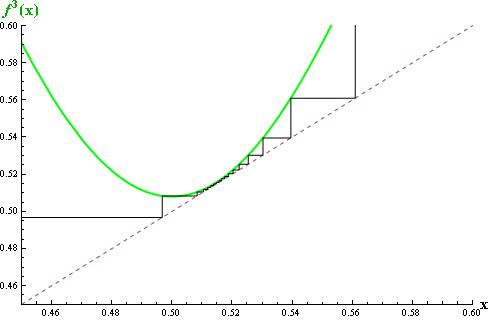
\includegraphics[width=0.9\textwidth]{235bcobwebdetaliu.jpg}\hspace*{\fill}
				
				\centering{\tiny \bf \color{darkblue} Detaliu ,,\textit{cobweb}'' intermiten\tb\ab.}
				
			\end{column}		
		\end{columns}
	
	
\end{frame}



%%%%%%%%%%%%%%%%%%%%%%%%%%%%%%%%%%%%%%%%%%%%%%%%%%%%%%%%%%%%%%%%%%%%%%%%%%%
%                                                                         %
%                       capitolul x:  Caracterizarea mecanismului de ,,\textit{folding}''                         %
%                                                                         %
%%%%%%%%%%%%%%%%%%%%%%%%%%%%%%%%%%%%%%%%%%%%%%%%%%%%%%%%%%%%%%%%%%%%%%%%%%%



%%%%%%%%%%%%%%%%%%%%% slide 9 %%%%%%%%%%%%%%%%%%%%%%%%%%%%%%%%%%%%%%


\section[Folding]{Caracterizarea mecanismului de ,,folding''}
\tableofcontents[currentsection,hideallsubsections]


\subsubsection{Analiza raportului $N^-_\delta/N^+_\delta$}
\begin{frame}
	\frametitle{Analiza raportului $N^-_\delta/N^+_\delta$}
	
	\begin{columns}[c]
		\begin{column}{0.5\textwidth}
			
			\hfill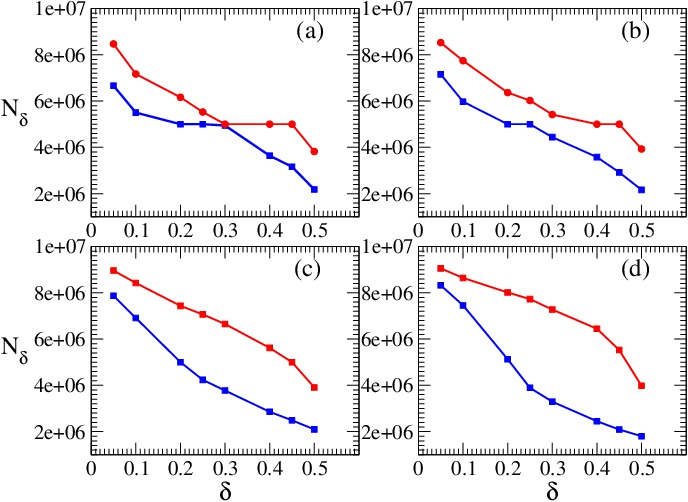
\includegraphics[width=0.7\textwidth]{N_abs_1}\hspace*{\fill}
			
			\centering{\tiny \bf \color{darkblue} $N_\delta$  ca func\tb ie de $\delta$, $\delta>0$  (albastru)
				si $\delta<0$ (ro\st u),  \\ $r$: (a) $3.60$; (b) $3.62$; (c) $3.67$; (d) $3.70$. }
			
			\hfill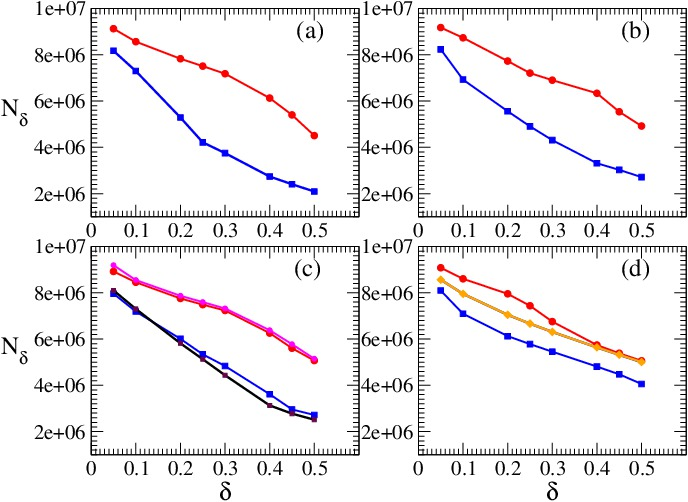
\includegraphics[width=0.7\textwidth]{N_abs_2}\hspace*{\fill}
			
			\centering{\tiny \bf \color{darkblue} $r$: (a)  $3.72$; (b) $3.77$; (c) $3.80$ \st i $3.82$; (d) $3.9$ \st i $4.0$. (La $r=4$ valorile sunt egale, portocaliu.) }
			
			
			
			
			
			
		\end{column}
		
		\begin{column}{0.5\textwidth}
			
			
			
			
			\hfill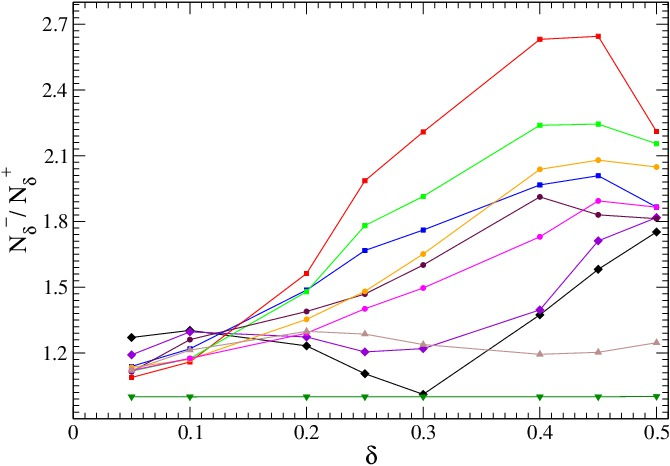
\includegraphics[width=0.65\textwidth]{fold_delta}\hspace*{\fill}
			
			\centering{\tiny \bf \color{darkblue} $N^-_\delta/N^+_\delta$  ca func\tb ie de $\delta$ la diferite valori fixate ale parametrului de control $r$ \ib n intervalul $[3.6,4]$: $r = 3.60$,$3.62$,$3.67$, $3.70$,$3.72$,$3.77$,$3.80$,$3.82$,$3.9$,$4.0$. }
			
			\hfill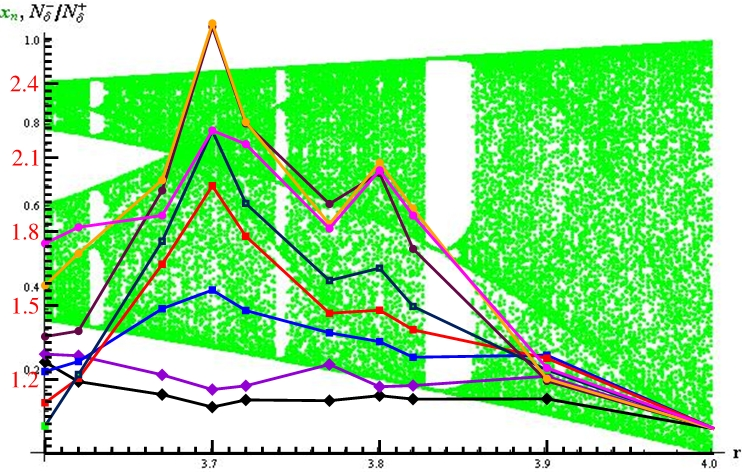
\includegraphics[width=0.7\textwidth]{ndeltapmorbit}\hspace*{\fill}
			
			\centering{\tiny \bf \color{darkblue} $N^-_\delta/N^+_\delta$  ca func\tb ie de parametrul de control $r$ la diferite valori fixate ale lui $\delta$ \ib n intervalul $(0,0.5]$: $\delta = 0.05$, $0.1$, $0.2$, $0.25$, $0.3$, $0.4$, $0.45$, $0.5$. }
			
		\end{column}
	\end{columns}
	
\end{frame}


%%%%%%%%%%%%%%%%%%%%slide X %%%%%%%%%%%%%%%%%%%%%%%%%%%%%%%%%%%%%%

\section[Concluzii]{Concluzii \hspace{43cm}}
%\tableofcontents[
%sectionstyle=show/hide,
%subsectionstyle=show/shaded/hide,
%subsubsectionstyle=show/show/hide/hide
%]
\begin{frame}\frametitle{Concluzii}

\begin{itemize}
	
	{\footnotesize
	\item 1. S-au introdus pentru prima dat\ab\ c\ac teva m\ab rimi fizice pentru caracterizarea mecanismului de \fol, care \ib mpreun\ab\ cu mecanismul de \str\ genereaz\ab\ dinamica haotic\ab: \nn, $\Gamma$, $N^-_\delta/N^+_\delta$
	
	}
\end{itemize}

\begin{itemize}
	
	{\footnotesize
		
		\item 2. S-a studiat comportamentul distan\tb ei medii asimptotice \dinf\ pe atractori stranii, demonstr\ac ndu-se c\ab\ este prima m\ab rime fizic\ab\ care la tranzi\tb ia la haos depinde ca func\tb ie de putere de ambele constante universale Feigenbaum
		\item 3. S-a aplicat pentru prima dat\ab\ metoda statisticii inverse \ib n studiul unui sistem determinist haotic: Caracterul universal al distribu\tb iilor pentru cazul ergodic, clas\ab\ de universalitate corespunz\ab toare exponentului critic $\approx-2.5$, senzitivitatea distribu\tb iilor fa\tb \ab\ de caracteristicile atractorilor stranii
	}
\end{itemize}

\end{frame}

\begin{frame}\frametitle{Concluzii}
	
		
	\begin{itemize}
		
		{\footnotesize
			
			\item 4. S-a extins metoda statisticii inverse \st i pentru un sistem dinamic complex, mai precis regiunea seismic\ab\ Vrancea, ob\tb in\ac ndu-se distribu\tb iile timpilor de a\st teptare pentru diferite valori de prag ale magnitudinii. Se constat\ab\ o evolu\tb ie a distribu\tb iei de la func\tb ie de putere cu un exponent $\approx-1.7$ spre o distribu\tb ie mai plat\ab\ a probabilit\ab \tb ilor timpilor de a\st eptare, ca \st i o asimetrie \ib ntre valorile pozitive \st i negative ale pragului, care reflect\ab o schimbare \ib n dinamica de producere a seismelor
		}
	\end{itemize}
	
\end{frame}



\end{document}
